\section{Materials}
    \subsection{Density}
        Density ($\rho$) is the amount of mass per unit of volumn of a material, thus it is given by the equation:
        \begin{equation}
            \rho=\frac{m}{V}
        \end{equation}
        Where $m$ is the mass of the object, and $V$ is the volume of the object.
        To measure the mass of an object, a balance is used.
        To measure the volume of the object, you can place the object into a filled Eureka can, which will overflow the can into a measuring cylinder, which can be used to measure the volume of displaced water, however this only works if the object is more dense than water ($\rho>1000\,\text{kg\,m}^{-3}$)

    \subsection{Stress, Strain and Young's Modulus}
        \subsubsection{Stress}
            Stress ($\sigma$) is how much force ($F$) is applied per unit of area ($A$).
            This means that little pressure over a small area is a similar stress to a large force spread over a large area.
            Stress has the formula:
            \begin{equation}
                \sigma=\frac{F}{A}
            \end{equation}
            Stress has the units $\text{N\,m}^{-2}\equiv\text{Pa}$.

        \subsubsection{Strain}
            Strain ($\varepsilon$) measures how much a material will stretch, relative to its initial size, under a force.
            It is given by the equation:
            \begin{equation}
                \varepsilon=\frac{\Delta\ell}{\ell}
            \end{equation}
            The notation $\ell$ is used here to mean length (and $\Delta\ell$ to mean change in length), as in how long a piece of wire is, since that is generally how stress and strain are though about, however this would also work for other objects.
            Since length ($\ell$) and change in length ($\Delta\ell$) both have the same units (m), strain has no unit, i.e. it is dimensionless; just a ratio of how far it stretches relative to how long it already was.

        \subsubsection{Young's Modulus}
            Young's modulus ($E$) measures how easy it is to elastically deform an object.
            Applying a stretching force to an object will cause it to deform by a length $\Delta\ell$, so measuring the change in length when a force is applied would give an indication oof how easy it is to deform, however this would not measure a property of the material.
            Because a larger object/an object that is longer to start with would allow a larger deformation for the same force, and an object with a greater surface area over which the force is applied would case less deformation, those parameters have to be accounted for to measure a property of the material rather than that of the specific object.
            This requires stress and strain, which divide by the area and unextended length respectively, allowing for a measurement of the material itself.
            The Young's modulus of a material combines both the stress and strain like so:
            \begin{equation}
                E=\frac{\sigma}{\varepsilon}=\frac{F\ell}{A\Delta\ell}
            \end{equation}
            This is a true measure of how easy it is to stretch the material, without being altered by the dimensions of the object.
            Since strain is dimensionless, the units of Young's modulus are the same as the units for stress, $\text{N\,m}^{-2}\equiv\text{Pa}$.
            Often, the order of magnitude of the Young's modulus of a material is around that of GPa, e.g. the Young's modulus of copper is $\approx110\text{ to }130\,\text{GPa}$.

        \subsubsection{Measuring Stress, Strain and Young's Modulus (Required Practical IV)}
            This experiment will be to determine the Young's modulus of a copper wire.

            To find the Young's modulus of the wire, we must find:
            \begin{itemize}
                \item The magnitude of a force exterted on the wire ($F$)
                \item The cross-sectional area of the wire ($A$)
                \item The unextended length of the wire ($\ell$)
                \item The change in length of the wire when the force is applied ($\Delta\ell$)
            \end{itemize}
            
            First for the simple ones; these are done before starting to apply forces to the wire:
            
            To find the unextended length of the wire, cut a length of wire, and clamp it securely to an end of a table that will be used for the experiment.
            On the other end, set up a pulley as shown (don't add any mass yet):

            \begin{figure} \label{fig:required_practical_iv}
                \begin{center}
                    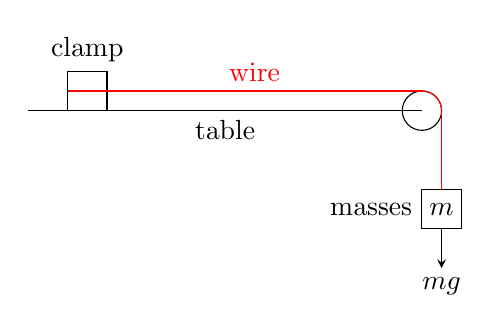
\begin{tikzpicture}
                        \draw (0,0) -- (5,0); % table
                        \draw (2.5,0) node[below]{table};
                        \draw (.5,0) rectangle (1,.5); % clamp
                        \draw (.75,.5) node[above]{clamp}; % clamp label
                        \draw (5,0) circle (.25); % pulley

                        \draw[red] (2.875,.25) node[above]{wire};
                        \draw[red] (.5,.25) -- (5,.25); % wire to pulley
                        \draw[red] (5,.25) arc[start angle=90, end angle=0, radius=.25];
                        \draw[red] (5.25,0) -- (5.25,-1);

                        \draw (5,-1) rectangle (5.5,-1.5);
                        \draw (5,-1.25) node[left]{masses};
                        \draw (5.25,-1.25) node{$m$};
                        \draw[-stealth] (5.25,-1.5) -- (5.25,-2);
                        \draw (5.25,-2) node[below]{$mg$};
                    \end{tikzpicture}
                \end{center}
                \caption{The setup for Required Practical IV}
            \end{figure}

            Then, use a metre (or longer) ruler or tape measure if appropriate to measure the length of the wire.
            The wire should be measured to at least the nearest cm, ideally the nearest mm.
            A longer wire is better, since that will cause a greater extension, which can be more easily measured to a greater degree of precision.

            To find the corss-sectional area of the wire, we must first find the diameter, and then use the formula:
            \begin{equation}
                A=\frac{\pi d^2}{4}
            \end{equation}
            To find the diameter, use a micrometer, since this will measure small distances (such as the diameter of a wire) to a high degree of precision.

            The other two measurements will now require exterting a force on the wire.
            Before adding any mass, set up a ruler measuring from the pulley in the direction of the clamp.
            Place a marker (such as a piece of tape) on the wire, hanging over the ruler.
            
            Then, put on safety goggles and securely clamp one end of the wire, then hang a 100\,g (0.1\,kg) mass on the other end of the pulley.
            Measure how far the marker has moved along the ruler.
            The repeat, adding more and more 100\,g weights to the wire and measuring how far the markers moves after each new weight.
            Keep adding weights until the wire snaps.
            The movements of the wire are likely to be on the order of millimetres.

            This is an example of the data collected:

            \begin{center}
                \begin{tabular}{c|c}
                    \textbf{Mass/kg} & \textbf{Extension/mm ($\pm$0.5\,mm)} \\
                    \hline
                    0.0 & 0 \\
                    0.1 & 1 \\
                    0.2 & 2 \\
                    0.3 & 4 \\
                    0.4 & 4 \\
                    0.5 & 5 \\
                    0.6 & 7 \\
                    0.7 & 8 \\
                    0.8 & 10 \\
                    0.9 & 16 \\
                    1.0 & 27
                \end{tabular}
            \end{center}

            At higher forces, the wire may begin to slip quite far after each new mass added.
            This is where the wire reaches plastic deformation, and these results should be ignored.

            Plot the results on a graph, which should look something like this (ignoring the final two anomalies):

            \begin{figure}
                \begin{center}
                    \begin{tikzpicture}[>=stealth]
                        \draw[->] (0,0) -- (5.5,0) node[right] {$m$};
                        \draw[->] (0,0) -- (0,5.5) node[above] {$\Delta\ell$};
                        \draw (0,0) node[below left]{0};

                        \draw (1,0) node[below]{0.2};
                        \draw (2,0) node[below]{0.4};
                        \draw (3,0) node[below]{0.6};
                        \draw (4,0) node[below]{0.8};
                        \draw (5,0) node[below]{1.0};

                        \draw (0,1) node[left]{6};
                        \draw (0,2) node[left]{12};
                        \draw (0,3) node[left]{18};
                        \draw (0,4) node[left]{24};
                        \draw (0,5) node[left]{30};

                        \pic[red] at (0,0) {cross};
                        \pic[red] at (0.16667,.5) {cross};
                        \pic[red] at (0.33333,1) {cross};
                        \pic[red] at (0.66667,1.5) {cross};
                        \pic[red] at (0.66667,2) {cross};
                        \pic[red] at (0.83333,2.5) {cross};
                        \pic[red] at (1.16667,3) {cross};
                        \pic[red] at (1.33333,3.5) {cross};
                        \pic[red] at (1.66667,4) {cross};
                        \pic[red] at (2.66667,4.5) {cross};
                        \pic[red] at (4.5,5) {cross};

                        \draw[red] (0,0.14106) -- (1.66667,4.22167); % LoBF calculated using a linear regression in Desmos
                        \draw[dashed,red] (0,0.14106) -- (2.18879,5.5); % Extrapolation

                        \draw (-1,2.5) node{\rotatebox{90}{Extension/mm}};
                        \draw (2.5,-1) node{Mass/kg};
                    \end{tikzpicture}
                \end{center}
                \caption{A graph of the results with a line of best fit}
            \end{figure}

            You could also add error bars and calculate a steepest and shallowest line of best fit.

            To find the Young's modulus from this graph, we can use the fact that we have a gradient representing $\frac{\Delta\ell}{m}$, which can be converted to $\frac{\Delta\ell}{F}$ by dividing by $g$.
            Then, using the formula for Young's modulus in terms of $\frac{\Delta\ell}{F}$, we can find the Young's modulus to be:
            \begin{equation}
                E=\frac{\ell}{A}\times\left(\frac{\Delta\ell}{F}\right)^{-1}
            \end{equation}
    \newpage